\chapter{Crystallization of the crust of a non-accreting neutron star}

% something pns
% crystallization temperature is a lower estimate for the temperature at which 
%   nuclear reactions fall out of equilibrium (see ic sh paper)
% most of the results presented in this Chapter are published

\minitoc\newpage

\section{Model of the crust at finite temperature}\label{sec:modelcrusttemp}

This section deals with the model of the crust at finite temperature. 
Since the possible contribution of a free proton gas is expected to be small at 
the temperatures considered, we neglect it. This working hypothesis 
is a posteriori confirmed by the calculation of the proton fugacity, 
$z_p = \exp[(\mu_p-m_pc^2)/(k_B T)]$, which never exceeds $-20$ MeV in 
the density and temperature domain of interest. 
The existence of nonspherical pasta phases expected in the deeper layers of the 
inner crust ($n_B \gtrsim 0.05$ fm$^{-3}$~\cite{Pearson2020}) is difficult to 
account for in the multicomponent plasma (MCP) approach~\cite{Barros2020}, and 
as a consequence is not considered in this study.

We review the one-component plasma (OCP) approximation 
in~\ref{subsec:ocp}. We give the expressions of the ideal and interacting
contributions to the ion free energy in solid and liquid phases, and discuss 
the thermodynamic condition for crystallization. The nuclear statistical
equilibrium (NSE) is implemented perturbatively in the MCP approach 
in~\ref{subsec:mcp}. The derivation of the rearrangement term, 
required to guarantee thermodynamic consistency, is carried out.
In~\ref{subsec:freeenfunctional}, we present the free energy functional used in
the free neutron regime.

\subsection{One-component Coulomb plasma approximation}\label{subsec:ocp}

At zero temperature, WS cells are supposed to be identical, thus the OCP  
(single-nucleus) approximation~\cite{Baus1980}, which considers a unique 
nucleus $(A,Z)$ for a given thermodynamic condition of pressure and temperature 
$(P,T)$, is exact. Let us recall that the equilibrium composition is 
determined by minimizing the Gibbs free energy per nucleon at fixed
pressure~\cite{Fantina2020} 
(or equivalently the free energy density at fixed baryon
density~\cite{Lattimer1991,Gulminelli2015,Carreau2019}).
At finite temperature in the OCP approximation, the expected distribution of 
nuclei is replaced by the equilibrium nucleus obtained from the minimization of 
the relevant thermodynamic potential.
The physical properties of the OCP are fully characterized by the so-called 
dimensionless Coulomb coupling parameter,
%
\begin{equation}
  \Gamma = \frac{Ze^2}{a_N k_B T},\label{eq:gamma}
\end{equation}
%
where $a_N=(4\pi n_N/3)^{-1/3}$ is the ion-sphere radius, $n_N=1/V_{WS}$ being 
the ion density.
More precisely, $\Gamma$ allows to quantify the nonideality of the system, that
is the importance of the many-body interactions in the OCP. The lower the
temperature, the more coupled are the ions. The crystallization of the OCP into 
a lattice is observed at $T=T_m$, corresponding to 
$\Gamma = \Gamma_m \approx 175$.

The total free energy per ion in the crust is given by
%
\begin{equation}
  F = F_{i,e} + F_g + F_e,\label{eq:fperion}
\end{equation}
%
where $F_{i,e}$ is the ion free energy in the e-cluster representation, 
see~\ref{subsec:nucenergy}, $F_g$ is the neutron gas free energy, and $F_e$ 
is the electron gas free energy, given by~\cite{Haensel2007}
%
\begin{equation}
  \mathcal{F}_e = \frac{F_e}{V_{WS}} = \varepsilon_e -
  \frac{P_r}{6}t_r^2x_r\gamma_r,\label{eq:fel}
\end{equation}
%
with $t_r = T/(m_e c^2)$. The expressions of the energy density 
$\varepsilon_e$, relativistic unit of the electron pressure $P_r$, relativity
parameter $x_r$, and $\gamma_r$ are given in~\ref{subsubsec:elgas}. It should
be stressed that Eq.~(\ref{eq:fel}) is obtained by employing a Sommerfeld
expansion in the limit $t_r \ll \gamma_r - 1$.
Let us notice that in the regime of the outer crust, neutrons are still bound
to the nuclei, thus $F_g=0$ MeV, and consequently $F_{i,e}$ coincides with the 
ion free energy in the r-cluster representation $F_i$.
The ion free energy reads
%
\begin{equation}
  F_{i,e} = M_{i,e} c^2 + F_i^{\text{id}} + F_i^{\text{int}},\label{eq:fie}
\end{equation}
%
where the ion mass in e-cluster representation $M_{i,e}$ has been introduced.
In Eq.~(\ref{eq:fie}), $F_i^{\text{id}}$ represents the ideal contribution to
the ion free energy, that is the noninteracting part, and $F_i^{\text{int}}$
the interacting part.

In the following, we give the expressions associated to the ideal and 
interacting contributions to the ion free energy which differ according to the 
phase of matter, either solid or liquid. In the free neutron regime, the 
finite-size contribution is included and is common to both phases. The latter 
is derived from the application of Gauss theorem,
%
\begin{equation}
  E_{fs} = \frac{2n_p}{n_0(1-I)}\frac{e^2}{r_0}\frac{Z^2}{A^{1/3}},
\end{equation}
%
where $r_0=(4\pi n_0/3)^{-1/3}$ is related to the average density of the
cluster $n_0$.
The modeling of $M_{i,e}$ as well as of the neutron gas free energy $F_g$ is 
presented in detail in~\ref{subsec:freeenfunctional}. 

\subsubsection{OCP in a liquid phase}

Above the crystallization temperature, $T > T_m$, the OCP is in a liquid phase.
In the Coulomb liquid, each ion can move freely within the volume of the WS 
cell in which it is confined. This translational center-of-mass motion is
accounted for in the noninteracting part of the ion free energy, which
therefore reads~\cite{Haensel2007}
%
\begin{equation}
  F_i^{\text{id}} = k_B T 
  \left[\ln\left(\frac{n_N\lambda^3}{g_s}\right) - 1\right]\label{eq:fliqid},
\end{equation}
%
where $g_s$ is the spin degeneracy, which we take $g_s=1$ for nuclei whose
ground-state angular momentum is unknown, and $\lambda$ is the de Broglie
wavelength of the component given by
%
\begin{equation}
  \lambda = \sqrt{\frac{2\pi(\hbar c)^2}{M_{i,e}c^2 k_B T}}.
\end{equation}
%

The interacting part of the ion free energy can be decomposed
as~\cite{Fantina2020}
%
\begin{equation}
  F_i^{\text{int}} = F_{ii,\text{liq}} +
  F_{ie,\text{liq}}^{\text{pol}}\label{eq:fiintliq}
\end{equation}
%
Analytical formulae have been derived for these two terms 
in~\cite{Potekhin2000}.
In the present study, we find that the importance of the correction
associated to electron polarization effects, 
$F_{ie,\text{liq}}^{\text{pol}}$ (Eq.~(19) of~\cite{Potekhin2000}), is very 
small in the density and temperature regime of interest, and is therefore 
neglected. The only significant effect of the latter correction is to change 
the crystallization temperature of $40-50\%$ around $P\approx 1.25\times 
10^{-4}$ MeV/fm$^3$, where the composition changes drastically due to 
shell structure~\cite{Fantina2020}.
For the total Coulomb contribution, we employ the parametrization 
proposed in~\cite{Potekhin2000}: 
%
\begin{eqnarray}
  \frac{F_{ii,\text{liq}}}{k_B T} 
  &=& A_1\left[\sqrt{\Gamma(A_2+\Gamma)} - A_2\ln\left(\sqrt{\Gamma/A_2} 
+ \sqrt{1+\frac{\Gamma}{A_2}}\right)\right]\notag\\
  &&+ 2A_3\left(\sqrt{\Gamma} - \arctan\sqrt{\Gamma}\right) 
  + B_1\left[\Gamma-B_2\ln\left(1+\frac{\Gamma}{B_1}\right)\right]\notag\\
  &&+ \frac{B_3}{2}\ln\left(1+\frac{\Gamma^2}{B_4}\right),
\end{eqnarray}
%
with $A_1=-0.9070$, $A_2=0.62954$, $A_3=-\sqrt{3}/2-A_1/\sqrt{A_2}$,
$B_1=4.56\times 10^{-3}$, $B_2=211.6$, $B_3=-10^{-4}$, and $B_4=4.62\times
10^{-3}$. Let us notice that the latter parametrization 
solely depends on the Coulomb coupling parameter $\Gamma$, 
Eq.~(\ref{eq:gamma}), and that $F_{ii,\text{liq}}$ vanishes at high 
temperature.

\subsubsection{OCP in a solid phase}

Once the crystallization temperature $T_m$ is reached, we assume that the OCP 
crystallizes into a perfect body-centered cubic lattice~\cite{Chamel2016}, as
in the zero temperature case studied in Chapter 1. In the solid OCP, ions are
able to oscillate near their equilibrium positions. Hence, the ideal 
part of the ion free energy accounting for the translational motion in the 
liquid OCP, $F_{i}^{\text{id}}$, is replaced by the zero-point motion energy, 
$E_{zp}$, Eq.~(\ref{eq:ezp}). The ion free energy in the e-cluster
representation is therefore rewritten as
%
\begin{equation}
  F_{i,e,\text{sol}} = M_{i,e}c^2 + E_{zp} + F_{ii,\text{sol}} +
  F_{ie,\text{sol}}^{\text{pol}},
\end{equation}
%
where $F_{ie,\text{sol}}^{\text{pol}}$ corresponds to the polarization
correction in the solid phase~\cite{Potekhin2000}, which is neglected here, and
$F_{ii,\text{sol}}$ is the Coulomb interaction term that can be decomposed as
%
\begin{equation}
  F_{ii,\text{sol}} = E_L + F_{\text{th}} + F_{\text{ah}} - k_B
  T\ln(g_s).\label{eq:fiisol}
\end{equation}
%
In the latter expression, $E_L$ represents the temperature-independent static 
lattice term, given by Eq.~(\ref{eq:eL}). The last term in~\ref{eq:fiisol} is
the spin entropy. As previously, we fix $g_s=1$ for nuclei whose spin 
degeneracy is unknown, yet the inclusion of this term has no effect on the 
determination of the crystallization temperature because it is the same for 
both liquid and solid OCP.

As for total Coulomb contribution in the liquid phase, the thermal
contribution due to the ion vibrations around their equilibrium position in the 
harmonic approximation and the anharmonic correction have been analytically
fitted by Baiko \textit{et al.}~\cite{Baiko2001} and Potekhin \&
Chabrier~\cite{Potekhin2010}, respectively. 
The expression employed for the thermal contribution reads~\cite{Baiko2001}
%
\begin{equation}
  \frac{F_{\text{th}}}{k_B T} = \sum_{n=1}^3\ln\left(1
    -\text{e}^{-\alpha_n\theta}\right) 
  - \frac{A(\theta)}{B(\theta)},
\end{equation}
%
where $\theta \equiv \hbar\omega_p/(k_B T)$, $\omega_p$ being the ion plasma
frequency, Eq.~(\ref{eq:omegap}), and
%
\begin{equation}
  A(\theta) = \sum_{n=0}^{8}a_n\theta^n,
\end{equation}
%
\begin{equation}
  B(\theta) = \sum_{n=0}^{7}b_n\theta^n 
  + \alpha_6 a_6 \theta^9 
  + \alpha_8 a_8 \theta^{11},
\end{equation}
%
with $\alpha_n$, $a_n$, and $b_n$ numerical constants (see Table II
in~\cite{Baiko2001}).
The analytical expression of the anharmonic correction used in our study
is~\cite{Potekhin2010}

\begin{equation}
  F_{\text{ah}} =
  F_{\text{ah}}^{(0)}\text{e}^{-c_1\theta^2} 
  - k_B T d_1\frac{\theta^2}{\Gamma},\label{eq:ah}
\end{equation}
%
where
%
\begin{equation}
  F_{\text{ah}}^{(0)} = k_B T\sum_{n \geq 1}\frac{f_n}{n\Gamma^n}
\end{equation}
%
with $c_1$, $d_1$, and $f_n$ numerical constants. One should stress that
the latter expression is modified with respect to that proposed by Farouki \&
Hamaguchi, $F_{\text{ah}}^{(0)}$, based on numerical simulations of 
the solid OCP for $170 \leq \Gamma \leq 2000$~\cite{Farouki1993}, so as to
reproduce the zero-temperature and classical limits.

\subsubsection{Crystallization of a OCP}

As in previous works~\cite{Fantina2020,Carreau2019,Carreau2020}, we compute 
the crystallization temperature within the OCP approximation, which is 
simple and not costly from the numerical point of view. An additional reason is
that the ion distribution  could be frozen at some temperature $T_f > T_m$ 
considering the present uncertainties on timescales relative to NS 
cooling~\cite{Goriely2011}.

\begin{figure}[!t]
  \begin{center}
    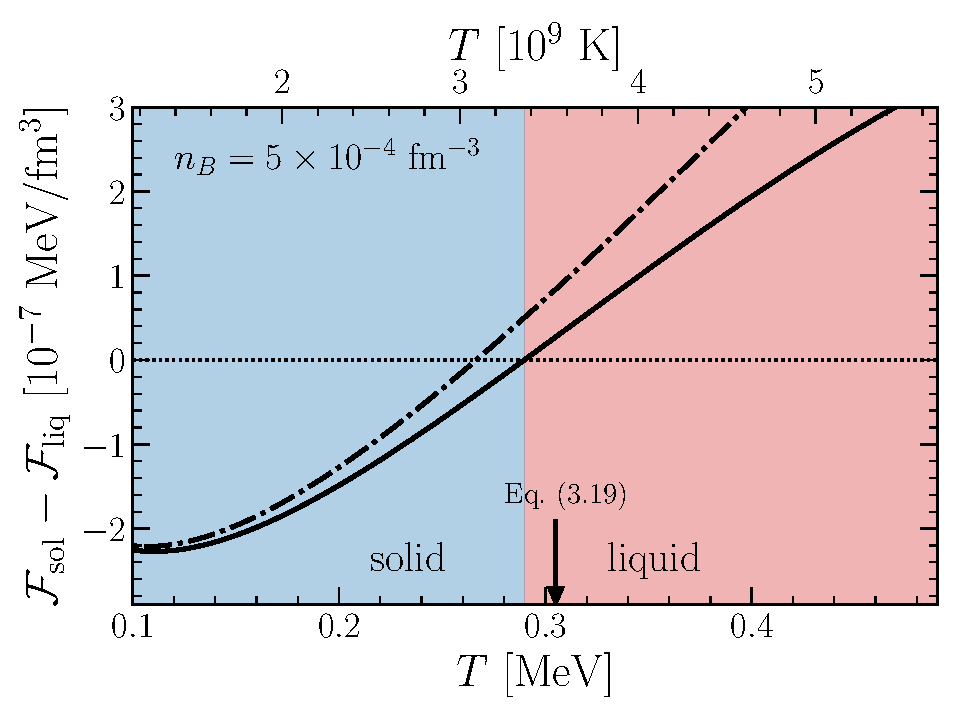
\includegraphics[width=0.9\linewidth]{figures/fliqsol.pdf}
  \end{center}
  \caption[Free energy density difference between liquid and solid phases
  versus temperature]{Variation with temperature $T$ of the free energy density
  difference between liquid and solid phases
$\mathcal{F}_{\text{sol}}-\mathcal{F}_{\text{liq}}$ for the optimal composition
$\bm{\theta_{\text{liq}}}$ at $n_B=5\times 10^{-4}$ fm$^{-3}$ (free neutron 
regime) with (solid line) and without (dashdotted line) the anharmonic
contribution, Eq.~(\ref{eq:ah}), to the free energy in the solid 
phase, using BSk24 CLDM. The crystallization temperature obtained from 
Eq.~(\ref{eq:tmapprox}) is also indicated.}\label{fig:fliqsol}
\end{figure}

The condition of crystallization of a OCP with associated composition 
$\bm{\theta}$ is 
%
\begin{equation}
  \mathcal{F}_{\text{liq}}(\bm{\theta}, T_m) 
  = \mathcal{F}_{\text{sol}}(\bm{\theta}, T_m),\label{eq:tmocp}
\end{equation}
%
where $\mathcal{F}_\text{liq}$ and $\mathcal{F}_\text{sol}$ are the WS cell
free energy density in the liquid and solid phase, respectively.
The latter equation is equivalent to
%
\begin{equation}
  F_i^{\text{id}} + F_{ii,\text{liq}} = E_{zp} + F_{ii,\text{sol}},
\end{equation}
%
which shows that the Coulomb coupling parameter at melting
temperature $\Gamma_m$ strongly depends on the corrections that step in a
finite temperature. Furthermore, those corrections are small in the vicinity
the crystallization temperature, making it difficult to estimate $\Gamma_m$
with precision. Still, several works estimate the Coulomb parameter to 
$\Gamma_m \approx 175$~\cite{VanHorn1969,Haensel2007}. 
The crystallization temperature of a OCP at a given baryon density $n_B$ 
can then be approximated by inverting Eq.~(\ref{eq:gamma}), yielding
%
\begin{equation}
  T_m \simeq \frac{(Ze)^2}{k_B a_N \Gamma_m} \ \text{K},\label{eq:tmapprox}
\end{equation}
%
assuming the composition to be the same as in CCM. 
%
We proceed as in~\cite{Fantina2020} in order to precisely calculate the 
crystallization temperature. At each value of the baryon density $n_B$ and 
temperature $T$, the equilibrium composition is computed following the 
procedure detailed in Chapter 1. Specifically, we solve the coupled 
differential equations, Eqs.~(\ref{eq:ic1})-(\ref{eq:ic4}), using the 
expressions of $F_{i}^{\text{id}}$ and $F_{i}^{\text{ind}}$ of the liquid 
phase, yielding the optimal liquid composition $\bm{\theta_{\text{liq}}}$ and 
the associated WS cell free energy density $\mathcal{F}_{\text{liq}}$. Then, 
for the same composition $\bm{\theta_{\text{liq}}}$, we calculate the free 
energy density assuming a solid phase 
$\mathcal{F}_{\text{sol}}(\bm{\theta_{\text{liq}}})$. The lowest temperature 
for which $\mathcal{F}_{\text{liq}} \geq \mathcal{F}_{\text{sol}}$ is 
identified as the crystallization temperature $T_m$ corresponding to the 
baryon density under study. The first guess for $T_m$ is obtained from the
application of Eq.~(\ref{eq:tmapprox}).

Fig.~\ref{fig:fliqsol} shows the variation with temperature of the free energy
difference $\mathcal{F}_{\text{sol}}-\mathcal{F}_{\text{liq}}$ at a given
baryon density $n_B = 5\times 10^{-4}$ for the BSk24 CLDM based on the 
metamodeling technique. The intersect of the solid line and zero marks
the crystallization temperature, $T_m = 0.29$ MeV, which is equivalent to $T_m
= (1.16\times 10^{10}) \times (0.29) = 3.36 \times 10^9$ K. We can observe that
the crystallization temperature is significantly lower if the 
anharmonic contribution to the free energy of the solid OCP is neglected 
(dashdotted line). This stresses the importance of the small thermal
corrections in the calculation. It is also seen that the effect of the 
anharmonic contribution becomes bigger with temperature increasing, and 
vanishes in case of strong coupling, that is in the zero-temperature limit. We
find that the simple expression Eq.~(\ref{eq:tmapprox}) gives a fairly good
estimation of the crystallization temperature.

\subsection{Multicomponent Coulomb plasma in a liquid phase}\label{subsec:mcp}

The OCP approximation is expected to be reliable at the temperatures
typically encountered at low density in the crystallized crust, yet the 
very principle of statistical mechanics tells us that at finite temperature 
different configurations of the WS cell are realized for a same total density.
In the following, the nuclear distribution is included in a MCP approach at 
equilibrium, as in~\cite{Fantina2020,Carreau2020}. A 
particular attention is paid to the evaluation of the chemical potentials, as 
well as of the rearrangement term, which is required to ensure thermodynamic 
consistency. 

\subsubsection{Nuclear statistical equilibrium}

% introducing MCP formalism
The NS crust at a given depth in the star is supposed to contain different ion
species characterized by their mass and charge number $(A^{(j)},Z^{(j)})$, 
associated to different WS cells of volume $V_{WS}^{(j)}$, such that $p_j$ is 
the frequency of occurence (or probability) of the component $(j)$, with 
$\sum_j p_j = 1$.
Thermodynamic quantities are defined in terms of the ion densities of the 
different species $n_N^{(j)}$, which are related to the probabilities $p_j$ 
through 
%
\begin{equation}
  n_N^{(j)}=\frac{p_j}{\langle V_{WS}\rangle}.\label{eq:nnj}
\end{equation}
%
where the average WS cell volume has been introduced,
%
\begin{equation}
  \langle V_{WS} \rangle = \sum_j p_j V_{WS}^{(j)},
\end{equation}
%
the notation $\langle\rangle$ indicating ensemble averages.
The different configurations $(A^{(j)},Z^{(j)})$ are associated with different
different baryon densities $n_B^{(j)}$, such that the total baryon density is
%
\begin{equation}
  n_B = \sum_j p_j n_B^{(j)}.
\end{equation}
%
Conversely, they share the same total pressure $P$ imposed by the hydrostatic 
equilibrium and the same background densities of electrons, $n_e^{(j)}=n_e$, 
and of free neutrons, $n_g^{(j)}=n_g$.
It is assumed that the charge neutrality is assured at the level of each cell,
implying that the proton density is the same in each cell, $n_p^{(j)}=n_p$, and
equal to the electron density, 
%
\begin{equation}
  n_e = n_p = \sum_j n_N^{(j)} Z^{(j)} =
  \frac{Z^{(j)}}{V^{(j)}}.\label{eq:chargeneut}
\end{equation}

% energetics
The free energy density of the MCP is given by
%
\begin{equation}
  \mathcal{F} = \sum_j n_N^{(j)} F^{(j)},
\end{equation}
%
where $F^{(j)}$ is the free energy per ion of a single component $(j)$ defined 
in Eq.~(\ref{eq:fperion}).
The probabilities $p_j$ and ion densities $n_N^{(j)}$ are calculated such as to
maximize the thermodynamic potential in the canonical ensemble. 
Because of the chosen free energy decomposition, we can observe that the 
free neutron and electron contributions to the free energy density, 
respectively $\mathcal{F}_g$ and $\mathcal{F}_e$, do not depend on $n_N^{(j)}$,
%
\begin{equation}
  \mathcal{F}\left(\left\{n_N^{(j)}\right\}\right) 
  = \mathcal{F}_{i,e}\left(\left\{n_N^{(j)}\right\}\right) 
  + \mathcal{F}_g + \mathcal{F}_e,
\end{equation}
%
with
%
\begin{equation}
  \mathcal{F}_{i,e} = \sum_j n_N^{(j)} F_{i,e}^{(j)}.
\end{equation}
%
This means that the variation can be performed on the ion part only, yielding
%
\begin{eqnarray}
  d\mathcal{F}_{i,e} &=& \sum_j \left(F_{i,e}^{(j)} + n_N^{(j)} \frac{\partial
  F_{i,e}^{(j)}}{\partial n_N^{(j)}}\right)dn_N^{(j)} \notag\\
                     &=& \sum_j \left(F_{i,e}^{(j)} + k_B T + n_N^{(j)}
                     \frac{\partial F_i^{(j),\text{int}}}{\partial
                   n_N^{(j)}}\right)dn_N^{(j)} \notag\\
  &=& \sum_j \left(\Omega_{i,e}^{(j)} + k_B T \ln
  n_N^{(j)}\right)dn_N^{(j)},\label{eq:dfi}
\end{eqnarray}
%
where the single-ion canonical potential has been introduced,
%
\begin{equation}
  \Omega_{i,e}^{(j)} = M_{i,e}c^2 + k_B T\ln\frac{(\lambda^{(j)})}{g_s^{(j)}} 
  + F_i^{(j),\text{int}} 
  + n_N^{(j)} \frac{\partial F_i^{(j),\text{int}}}{\partial n_N^{(j)}}.
  \label{eq:omega}
\end{equation}
%
% discussion on the breaking of linear-mixing rule
A deviation to the linear-mixing rule (the hypothesis of uncorrelated WS 
cells) is observed in Eq.~(\ref{eq:omega}) due to the translational degree of 
freedom in the liquid phase~\cite{Gulminelli2015}, because within the MCP 
approach the center-of-mass position of each ion is not confined to the single 
cell volume $V_{WS}^{(j)}$ but can freely explore the whole volume. As a 
consequence, the average composition of the MCP does not coincide with the OCP 
optimal configuration in general.

% conservation laws
In Eq.~(\ref{eq:dfi}), the variations $dn_N^{(j)}$ are not independent because 
of the normalization of probabilities, and the baryon number and charge 
conservation laws:
%
\begin{eqnarray}
  \frac{1}{\langle V\rangle} &=& \sum_j n_N^{(j)},\label{eq:normp}\\
  n_B - n_g &=& 
  \sum_j n_N^{(j)} A^{(j)}
  \left(1-\frac{n_g}{n_0^{(j)}}\right),\label{eq:barcons}\\
  n_p &=& \sum_j n_N^{(j)} Z^{(j)}\label{eq:charcons}.
\end{eqnarray}
%
We can identify the mass number associated to component $(j)$ in e-cluster 
representation $A_e^{(j)}$ in the right hand side of Eq.~(\ref{eq:barcons}).
Let us recall that in the regime of the outer crust, $n_g = 0$ fm$^{-3}$ thus
$A_e^{(j)} = A^{(j)}$. The average density of the ion $(j)$ $n_0^{(j)}$ is
obtained by solving numerically the equation corresponding to the pressure 
equilibrium between the ion and the gas (see~\ref{subsec:formalism} for the 
derivation),
%
\begin{equation}
  \frac{n_0^{(j)}}{A^{(j)}}\frac{\partial F_i^{(j)}} {\partial n_0^{(j)}} 
  = P_g,
\end{equation}
%
$P_g$ being the pressure of the neutron gas, whose expression is given in 
Eq.~(\ref{eq:phm}). As in~\cite{Grams2018}, the neutron gas density is taken to 
be the OCP solution, $n_g = n_g^{\text{OCP}}$.
% pj definition
The constraints Eqs.~(\ref{eq:normp})-(\ref{eq:charcons}) are taken into 
account by introducing the Lagrange multipliers $\alpha$, $\mu_n$, and $\mu_p$, 
leading to the following equations for the equilibrium densities $n_N^{(j)}$:
%
\begin{eqnarray}
  \sum_j \left(\Omega_{i,e}^{(j)} + k_B T \ln n_N^{(j)} 
  - \alpha\right)dn_N^{(j)} 
  - \mu_n \sum_j N_e^{(j)}dn_N^{(j)} - \mu_p \sum_j Z^{(j)} dn_N^{(j)}  
  = 0
\end{eqnarray}
%
with $N_e^{(j)} = A_e^{(j)} - Z^{(j)}$.
Considering independent variations, the solutions are given by
%
\begin{equation}
  p_j = \mathcal{A}\exp\left(-\frac{\tilde{\Omega}_{i,e}^{(j)}}{k_B
  T}\right),\label{eq:pj}
\end{equation}
%
with the normalization constant
%
\begin{equation}
  \mathcal{A} = \exp\left(\frac{\alpha}{k_B T}\right) = \sum_j
  \exp\left(-\frac{\tilde{\Omega}_{i,e}^{(j)}}{k_B T}\right).
\end{equation}
%
The single-ion grand-canonical potential reads
%
\begin{equation}
  \tilde{\Omega}_{i,e}^{(j)} = \Omega_{i,e}^{(j)} - \mu_n N_e^{(j)} -
  \mu_p Z^{(j)},
\end{equation}
%
where $\mu_n$ and $\mu_p$ correspond finally to the neutron and proton 
chemical potentials, respectively. Let us note that the rest-mass energies are 
included in the the chemical potentials since they are contained in the ion 
free energy. 
% pj requires the evaluation of the rearrangement term as well as of the
%   neutron and proton chemical potentials
The calculation of the grand-canonical potential $\tilde{\Omega}_{i,e}^{(j)}$, 
entering the definition of the probabilities $p_j$, requires the 
evaluation of the chemical potentials $\mu_n$ and $\mu_p$, as well as of the 
rearrangement term
%
\begin{equation}
  \mathcal{R}^{(j)} = n_N^{(j)} 
  \frac{\partial F_i^{(j),\text{int}}}{\partial n_N^{(j)}},
\end{equation}
%
which are discussed thoroughly in~\ref{subsubsec:chempoteval}
and~\ref{subsubsec:rear}, respectively.

\subsubsection{Evaluation of the chemical
potentials}\label{subsubsec:chempoteval}

% expressions for mun and mup
For a given thermodynamic condition of pressure $P$ and temperature $T$, the
expression of the chemical potentials $\mu_n$ and $\mu_p$ can be derived from 
the well-known thermodynamic relation $\mathcal{F} + P = \mu_n n_n + \mu_p n_p 
+ \mu_e n_e$ together with the beta equilibrium condition $\mu_n = \mu_p + 
\mu_e$,
%
\begin{equation}
  \mu_n = \frac{\mathcal{F} + P}{n_B} \quad \text{and} \quad
  \mu_p = \mu_n - \frac{\mathcal{F}_e + P_e}{n_p},\label{eq:munmup}
\end{equation}
%
where the electron chemical potential and pressure, respectively $\mu_e$ and
$P_e$ have been introduced.
% how to normally solve the problem
The determination of the equilibrium probabilities $p_j$ within the complete 
NSE formalism therefore requires to solve a complex nonlinear system of coupled 
equations, which is obviously numerically costly. Still, the implementation of 
the complete NSE was carried out in different studies in recent
years~\cite{Oertel2017,Burgio2018}, in which simplified nuclear functionals 
were adopted, density was imposed instead of the pressure, and the 
rearrangement term was neglected.

% perturbative implementation of NSE (update the chemical potentials)
We choose here to implement the NSE perturbatively, as proposed 
in~\cite{Grams2018}. 
The motivation for this option comes from the recent work of Fantina 
\textit{et al.}, where a very fast convergence of the chemical potentials is 
observed, along with a reduction of the computational time and an increase of
the numerical precision~\cite{Fantina2020}.
% explain how we proceed
We start by solving the OCP variational equations in order to get the 
equilibrium composition, which gives a first guess for the chemical potentials,
$\mu_n^{\text{OCP}}$ and $\mu_p^{\text{OCP}}$, via Eq.~(\ref{eq:munmup}). 
The probabilities $p_j$ can then be evalulated using Eq.~(\ref{eq:pj}), and an
improved estimation of the chemical potentials $\mu_n$ and $\mu_p$ is
calculated via
%
\begin{equation}
  \mu_n = \frac{\sum_j n_N^{(j)}F^{(j)}}{\sum_j n_N^{(j)}A_e^{(j)} + n_g} +
  \frac{P}{n_B} \quad \text{and} \quad
  y_p\mu_e = \frac{\sum_j n_N^{(j)}F_e^{(j)}}{\sum_j n_N^{(j)}A_e^{(j)} + n_g} 
  + \frac{P_e}{n_B},
\end{equation}
%
where the average proton fraction of the mixture $y_p=\langle
Z\rangle/(n_B\langle V_{WS}\rangle)$ has been introduced, with 
$\langle Z \rangle = \sum_j p_j Z^{(j)}$. The problem is thus solved by
iteration until the convergence of the chemical potentials is observed. The
convergence criterion is reasonably set to be $\Delta \mu_n < 10^{-9}$ MeV
between iterations.
We find that the number of iterations required to achieve convergence never 
exceeds 3. The reason is that the OCP result for $\mu_n$ and $\mu_p$ is 
already very close to the actual solutions for all pressures and 
temperatures explored in this work. Therefore, while we do solve the 
self-consistent problem in the regime of the outer crust to calculate the 
chemical potentials, the OCP estimation is safely kept in the free neutron 
regime so as to drastically reduce the computational cost. Indeed, in doing so 
the MCP calculation becomes equivalent to the much simpler OCP one.

\subsubsection{Evaluation of the rearrangement term}\label{subsubsec:rear}

At a given thermodynamic condition $(P,T)$, the rearrangement term entering 
Eq.~(\ref{eq:omega}) requires to be evaluated if one wants to compute the ion 
abundancies through Eq.~(\ref{eq:pj}).
As already discussed in~\cite{Fantina2020}, the rearrangement term arises from 
the self-consistency induced by the Coulomb part of the ion free energy. This 
stems from the fact that, due to the strong incompressibility of the electrons, 
the condition of charge neutraly has been imposed at the level of each cell, 
see Eq.~(\ref{eq:chargeneut}), in contrast with the baryon density $n_B$ that 
can fluctuate from cell to cell, see Eq.~(\ref{eq:barcons}). 
In consequence, any component of the free energy density that depends on the 
local cell proton density $n_p^{(j)} = n_p$ leads to a dependence on the local 
density $n_N^{(j)}$ through Eq.~(\ref{eq:chargeneut}). With our presciption for 
the WS cell free energy, this is only the case for the interacting part 
$F_i^{(j),\text{int}}$. We can therefore rewrite the rearrangement term of 
component $(j)$ as
%
\begin{eqnarray}
  \mathcal{R}^{(j)} 
  &=& n_N^{(j)} \left.\frac{\partial F_i^{(j),\text{int}}}{\partial
    n_N^{(j)}}\right|_{\{n_N^{(j)}\}_{i\neq j}}
    = n_N^{(j)} \frac{\partial F_i^{(j),\text{int}}}{\partial n_p}
    \frac{\partial n_p}{\partial n_N^{(j)}}\notag\\
  &=& n_N^{(j)} Z^{(j)} \frac{\partial F_i^{(j),\text{int}}}{\partial n_p}.
\end{eqnarray}
%
The complication of the self-consistent resolution of Eq.~(\ref{eq:pj}) can be 
avoided by imposing the most probable ion in the MCP mixture to coincide with 
the OCP result, if nonlinear mixing terms are omitted~\cite{Grams2018}. 
This approximation for the rearragement term is justified by the principle of 
ensemble equivalence in the thermodynamic limit~\cite{Gulminelli2015}.

% the minimization
The maximum probability corresponds to the minimum of the single-ion
grand-canonical potential $\tilde{\Omega}_{i,e}$. We therefore minimize the 
single-ion grand-canonical potential with respect to $A$, $I=1-2Z/A$, and 
$n_0$ ($n_p$ and $n_g$ are fixed at a given thermodynamic condition), yielding 
the following nonlinear system of coupled equations:
%
\begin{eqnarray}
  \frac{n_0^2}{A}\left(\frac{\partial F_i}{\partial n_0} + \frac{\partial
  \mathcal{R}}{\partial n_0}\right) &=& P_g\label{eq:r1}\\
  \frac{2}{A}\left(\frac{\partial F_i}{\partial I} + \frac{\partial
  \mathcal{R}}{\partial I}\right) &=& \mu_n - \mu_p\label{eq:r2}\\
  \frac{\partial F_i}{\partial A} + \frac{\partial \mathcal{R}}{\partial A} +
  \frac{1-I}{A}\left(\frac{\partial F_i}{\partial I} + \frac{\partial
  \mathcal{R}}{\partial I}\right) &=& \mu_n - \frac{P_g}{n_0},\label{eq:r3}
\end{eqnarray}
%
where the partial derivatives are calculated at the values corresponding to 
the equilibrium OCP solution, with nonlinear mixing terms being excluded.
%
The comparison of Eqs.~(\ref{eq:r1})-(\ref{eq:r3}) with
Eqs.~(\ref{eq:ic2})-(\ref{eq:ic4}) indicates that $\mathcal{R}^{(j)}$ should 
not depend on $n_0^{(j)}$, meaning that $R^{(j)}=R^{(j)}(A^{(j)},Z^{(j)})$. In 
addition, the rearrangement term should verify the following equation at the 
OCP solution:
%
\begin{equation}
  \frac{1-I}{A}\frac{\partial \mathcal{R}}{\partial I} = -\frac{\partial
  \mathcal{R}}{\partial A},
\end{equation}
%
which is satisfied if $R^{(j)}$ linearly depends on 
$Z^{(j)} = A^{(j)} (1-I^{(j)})/2$. Our final expression for the rearrangement 
term is therefore
%
\begin{equation}
  \mathcal{R}^{(j)} \simeq Z^{(j)} \left\langle \langle n_N^{(j)}\rangle 
    \frac{\partial F_i^{(j),\text{int}}}{\partial n_p}\right\rangle_j
  = \frac{Z^{(j)}}{V_{WS}^{\text{OCP}}}
  \left.\frac{\partial F_i^{\text{int}}}{\partial n_p}\right|_{\text{OCP}},
\end{equation}
%
where $V_{WS}^{\text{OCP}}$ is the equilibrium OCP cell volume, and the
derivative is evaluated numerically at the OCP solution.

\subsection{Free energy functional in the free neutron 
regime}\label{subsec:freeenfunctional}

% in the regime of the outer crust, we make use of exp data
As previously discussed in Chapter 1, in the regime of the outer crust we use 
the present day knowledge on experimental masses of neutron rich 
nuclei~\cite{Huang2017,Welker2017}, combined with state-of-the-art 
microscopic HFB theoretical mass tables~\cite{Goriely2013}. The ion mass 
$M_{i,e}$ in the outer crust is therefore simply calculated using 
Eq.~(\ref{eq:ionmass}).

% ion mass in the inner crust
In the regime of the inner crust, $n_B \gtrsim 2.6 \times 10^{-4}$ fm$^{-3}$, 
we have seen that the ions are immersed in a neutron gas, whose free energy 
density $\mathcal{F}_g$ enters the expression of the ion mass in the e-cluter 
representation,
%
\begin{equation}
  M_{i,e}^{(j)} c^2 = (A^{(j)} - Z^{(j)})m_n c^2 + Z^{(j)} m_p c^2 
  + F_{cl}^{(j)} - \frac{A^{(j)}}{n_0^{(j)}}(\mathcal{F}_g + n_g m_n c^2),
\end{equation}
%
where $F_{cl}^{(j)}$ represents the nuclear free energy.
In the range of densities corresponding to the free neutron regime, the 
clusters are so neutron rich that experimental data are not available. As a 
consequence, the modeling of $F_{cl}^{(j)}$ is required.

% plan
In the following, we first recall the simple case of free Fermi gas before
deriving the expressions required to describe to the ambient neutron gas at 
finite temperature. 
We then give the expressions of the different quantities entering the 
expression of the smooth part of the nuclear free energy functional 
$F_{cl}^{(j)}$. The temperature dependence of shell corrections and its effect 
on the crystallization temperature is investigated in~\ref{subsec:shtemp}.

\subsubsection{Thermodynamics of nuclear matter}

Let us first consider a collection of noninteracting fermions. In the 
grand-canonical ensemble, it obeys Fermi-Dirac statistics and the average 
number of fermions occupying a single-particle state $i$ is given by the 
Fermi-Dirac distribution, 
%
\begin{equation}
  \langle n_i \rangle 
  = \left[1+\exp\left(\frac{e_i-\mu}{k_B T}\right)\right]^{-1},
\end{equation}
%
where $e_i$ is the energy of the single-particle state $i$, and $\mu$ is the
total chemical potential.
At the thermodynamic limit, the sum over states $i$ is replaced by an integral
over the energy, thus the Fermi-Dirac function that describe the
occupation rate of state of given energy $e$ is introduced,
%
\begin{equation}
  f_{\text{FD}}(e, T, \mu) 
  = \left[1+\exp\left(\frac{e-\mu}{k_B T}\right)\right]^{-1}.\label{eq:fFD}
\end{equation}
%
When replacing the sum by an integral, one need to introduce the density of
energy states $\rho(e)$. For a spinless free particle of energy $e=\hbar^2 
k^2/(2m)$, the density of states is given by $\rho(\vec{k}) =
\frac{V}{(2\pi)^3}$, with $k$ the wave vector and $V$ the volume. Using the 
relation $\rho(\vec{k})d^3k = \rho(e)de$, one obtains
%
\begin{equation}
  \rho(e) = g\frac{V}{4\pi^2}\left(\frac{2m}{\hbar^2}\right)^{3/2}\sqrt{e},
\end{equation}
%
where the spin degeneracy $g=2s+1$ (for fermions, $s=1/2$) has been introduced, 
and mass $m$ is the mass of a particle.
At the thermodynamic limit, that is if we consider a huge number of particles
at a given temperature $T$ so that a large number of states are occupied, all
ensembles are equivalent. This means that we can use the expressions of 
the grand-canonical ensemble to calculate for instance the exact number of 
particles and the energy, respectively
%
\begin{equation}
  N = \sum_i\langle n_i\rangle \simeq \int_0^\infty
  \rho(e)f_{\text{FD}}(e)de
  \quad \text{and} \quad 
  E \simeq \int_0^\infty e \rho(e) f_{\text{FD}}(e)de.\label{eq:stats_N}
\end{equation}
%

% zero temperature
At zero temperature, states are populated up to the Fermi energy $\mu(T=0) =
e_F$. Indeed, $f_{\text{FD}} = 1$ for $e < \mu$, otherwise $f_{\text{FD}} = 0$, 
which allows us to rewrite Eq.~(\ref{eq:stats_N}) as
%
\begin{equation}
  N(T=0) = \int_0^{e_F} de\rho(e),
\end{equation}
%
yielding the expression of the Fermi energy,
%
\begin{equation}
  e_F = \frac{\hbar^2}{2m}\left(3\pi^2\frac{N(T=0)}{V}\right)^{2/3} =
  \frac{\hbar^2 k_F^2}{2m},
\end{equation}
%
with $k_F=(3\pi^2N(T=0)/V)^{1/3}$ the Fermi wave vector.
At $T=0$ K, the free energy is simply equivalent to the energy:
%
\begin{equation}
  F(T=0) = E(T=0) = \int_0^{e_F} e\rho(e)de = \frac{3}{5}Ne_F.
\end{equation}
%

At nonzero temperature, the calculation of thermodynamic properties of a free
Fermi gas generally requires the numerical evaluation of Fermi integrals,
%
\begin{equation}
  F_\nu(u) = \frac{1}{\Gamma(\nu+1)}\int_0^\infty\frac{t^\nu}{1+\exp(t-u)}dt,
\end{equation}
%
where $\Gamma(\nu) = (\nu-1)!$ is the gamma function.
It is however useful to apply Sommerfeld development in the limit $T \ll
e_F$ -- which is satisfied in the range of temperatures explored in our work -- 
in order to derive analytical formulas. In that case, we can obtain the
expression of the chemical potential from $N=\int_0^\infty
\rho(e)f_{\text{FD}}(e)de$, assuming that $\mu=e_F(1+\alpha T^2)$. By
identifying terms scaling as $T^2$, we get
%
\begin{equation}
  \mu = e_F\left[1 - \frac{\pi^2}{12}\left(\frac{T}{e_F}\right)^2\right].
\end{equation}
%
We can proceed in the same manner to calculate the energy at finite
temperature and the entropy, respectively
%
\begin{equation}
  E = \frac{3}{5} N e_F 
  \left[1+\frac{5\pi^2}{12}\left(\frac{T}{e_F}\right)^2\right] \quad \text{and}
  \quad S = \frac{\pi^2}{2}N\frac{T}{e_F},
\end{equation}
%
which finally gives, using the thermodynamic relation $F=E-TS$, the expression
of the free energy of a nonrelativistic free Fermi gas,
%
\begin{equation}
  F = \frac{3}{5} N e_F
  \left[1-\frac{5\pi^2}{12}\left(\frac{T}{e_F}\right)^2\right].
\end{equation}
%

We now turn to show that those results can still be used in the case of 
a huge number of interacting fermions in a infinite volume at a finite density, 
that is for infinite nuclear matter. The energy density $\mathcal{H} =
\mathcal{K} + \mathcal{V}$ for this idealized system can be derived from an
effective functional, and is often decomposed into a kinetic term and a 
contribution due to the nuclear interactions, respectively $\mathcal{K}$ and 
$\mathcal{V}$.
As discussed in~\ref{subsubsec:hnm}, the effective mass $m_q^*$ of species $q$ 
is usually introduced to regroup in a single term of kinetic energy the 
momentum dependence of the mean field,
%
\begin{equation}
  \frac{\hbar^2 k_q^2}{2m_q^*} = \frac{\hbar^2 k_q^2}{2m_q} +
  U_{\text{eff}}(k_q).
\end{equation}
%
In the grand-canonical ensemble, the occupation rate of state of given energy
$e_q$ for interacting fermions reads
%
\begin{equation}
  f_q(e_q+U_q, T, \mu_q) 
  = \left[1+\exp\left(\frac{e_q + U_q - \mu_q}{k_B T}\right)\right]^{-1},
\end{equation}
%
where $e_q + U_q = \hbar^2 k_q^2/(2m_q^*) + U_q$ is the single-particle energy
of species $q$, $U_q = \partial\mathcal{H}/\partial n_q$ being the local mean
field potential, which is given in the metamodel by ($q=n,p$)
%
\begin{eqnarray}
  U_q &=& v_{MM}(n,\delta) + \frac{1+3x}{3}\left(\frac{\partial
  v_{MM}}{\partial x}\right)_{\delta}
  + (\tau_3 - \delta) 
  \left(\frac{\partial v_{MM}}{\partial \delta}\right)_x\notag\\
      &&+ (1+3x)\sum_{l=n,p}\frac{3}{5}\frac{1+\tau_{3,l}\delta}{2}
      e_{F,l}\left[1-\frac{5\pi^2}{12}\left(\frac{T}{e_{F,l}}\right)^2\right]
      \notag\\
      &&\times \frac{m_l^*}{m} \left[
        \kappa_{sat}+\tau_{3,l} \kappa_{sym} \left(\delta
        + \frac{\tau_3-\delta}{1+3x}\right)
    \right],
\end{eqnarray}
%
with $\tau_{3,l} = 1$ ($\tau_{3,l} = 1$) for $l=n$ ($l=p$). The expressions of
the potential energy $v_{MM}$ and effective masses are given 
in~\ref{subsubsec:hnm}. The simple case of free Fermi gas is recovered by 
introducing the effective chemical potential $\tilde{\mu}_q = \mu_q - U_q$,
yielding the free energy per particle of nuclear matter,
%
\begin{equation}
  f_{HM}(n,\delta,T) = \sum_{q=n,p}
  \frac{3}{5}\frac{1+\tau_3\delta}{2}e_{F,q}\left[
  1-\frac{5\pi^2}{12}\left(\frac{T}{e_{F,q}}\right)^2\right] +
  v_{MM}(n,\delta).\label{eq:freehm}.
\end{equation}
%
which enters the expression of the neutron gas free energy, $\mathcal{F}_g =
n_g f_{HM}(n_g,1,T)$.
Let us note that the chemical potential does not include the rest mass energy 
in the above expressions.

\subsubsection{Energetics of clusters at finite temperature in the CLD
approximation}

Within the CLD approximation, the nuclear free energy $F_{cl}$ at temperature 
$T$ of a cluster of mass number $A$, isospin asymmetry $I$, and average density 
$n_0$, can be decomposed into a bulk, surface and Coulomb part as
%
\begin{equation}
  F_{cl}^{CLD} = A f_{HM}(n_0,I,T) + F_{surf} + F_{curv} + F_{Coul},
\end{equation}
%
where $f_{HM}(n_0, I, T)$ represents the free energy per baryon of bulk nuclear
matter, which is calculated using Eq.~(\ref{eq:freehm}).
The expressions used for the surface and curvature free energy are given
in Eqs.~(\ref{eq:esurf}) and~(\ref{eq:ecurv}) respectively, with the exception
of the surface tension, Eq.~(\ref{eq:sigma}) whose expression is modified with 
respect to the zero temperature case in order to effectively account for the 
excitation of surface modes:
%
\begin{equation}
  \sigma(I,T) = \sigma(I, T=0)h(T), 
\end{equation}
%
with $h(T>T_c) = 0$ and $h(T \leq T_c) = [1-(T/T_c)^2]^2$ (see Eq.~(2.31)
of~\cite{Lattimer1991}).
However, because the critical temperature $T_c$ is of the order of 
$T_c \approx 1.75 \times 10^{11}$ K and the crystallization temperature is 
lower than $10^{10}$ K in the inner crust~\cite{Haensel2007}, $h\approx 1$ and 
the excitation of surface modes can be neglected.
Assuming spherical clusters, we write the Coulomb energy as
%
\begin{equation}
  F_{Coul} = \frac{3}{5}\frac{e^2}{r_0^2}\frac{Z^2}{A^{1/3}}.
\end{equation}
%

We limit ourselves to the empirical parameters 
associated to four different functionals of the BSk family taken 
from~\cite{Goriely2013}: BSk22, BSk24, BSk25, and BSk26.
We choose these models because they all provide excellent fits to the 
AME2016~\cite{Huang2017}, are compatible both with ab initio and NS mass 
constraints, and explore a relatively large domain in the symmetry energy 
parameters (consistent with existing experimental constraints), which 
constitute the most important part of the EoS 
uncertainty~\cite{Pearson2014,Pearson2018}. Moreover, for each functional, 
surface and curvature parameters can be fitted to the ETF 
results~\cite{Pearson2019}, and the corresponding Strutinsky shell corrections, 
which are tabulated in~\cite{Pearson2018}, can be added on top of the CLD free 
energy, see~\ref{subsec:strutinsky} and~\ref{subsec:shtemp}.
Another motivation is that full mass tables obtained by deformed HFB 
calculations have been published for these models~\cite{Xu2013} and can 
therefore be used in the regime of the outer crust as a
complement to experimental masses~\cite{Fantina2020}.

\section{Study of the outer crust at crystallization}

In this section, we present the results for the outer crust at finite
temperature, and more at crystallization.
% what is included by default
Unless explicitly stated, all thermal corrections introduced in
Section~\ref{sec:modelcrusttemp} are included in the ion free energy.
% exp data when available
We made use of experimental masses from AME2016 \cite{Huang2017} when 
available, apart from the mass excesses of $^{77-79}$Cu which are better 
constrained in~\cite{Welker2017}.

The crystallization temperature of a OCP is calculated throughout the outer
crust in~\ref{subsec:tm_ocrust}. In~\ref{subsec:compo_ocrust_tm}, the
equilibrium composition of the MCP at crystallization is presented, and 
deviations with respect to CCM are investigated. The variation with pressure of 
the impurity parameter is analyzed in~\ref{subsec:qimp_ocrust}. Finally, the 
fraction of odd nuclei present in the outer crust at crystallization is 
computed in~\ref{subsec:odd_ocrust}.

\subsection{Crystallization temperature}\label{subsec:tm_ocrust}

\begin{figure}[!t]
  \begin{center}
    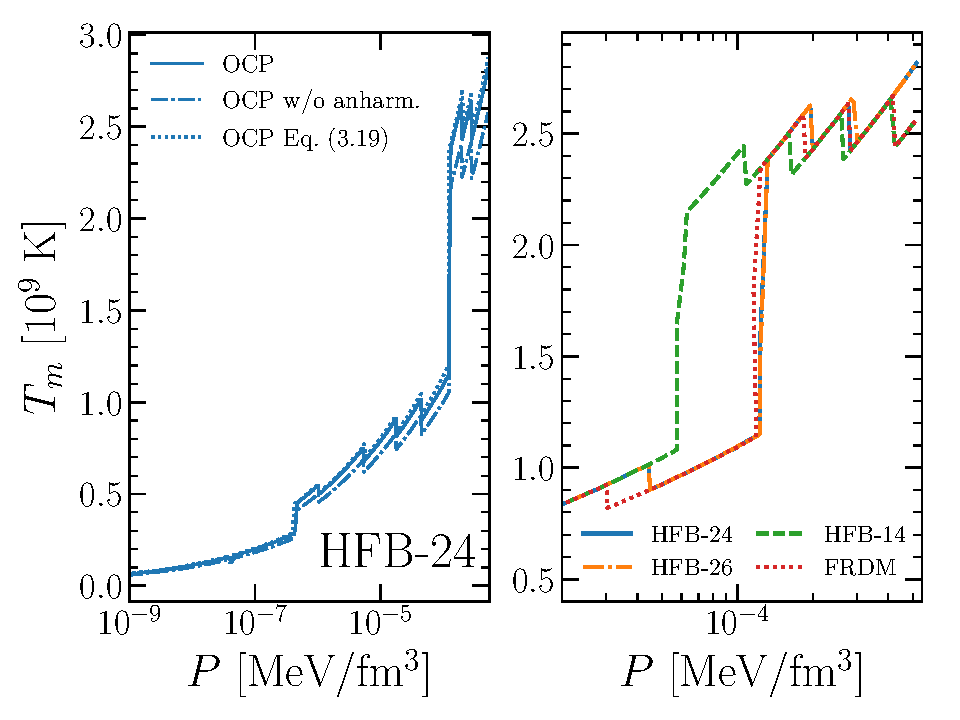
\includegraphics[width=0.9\linewidth]{figures/tm_ocrust.pdf}
  \end{center}
  \caption[Crystallization temperature versus pressure for the one-component 
  plasma in the outer crust]{Crystallization temperature $T_m$ as a function of
    pressure $P$ for the OCP in the outer crust. The left panel shows $T_m$ 
    for the  OCP with all corrections included (solid line), without 
    taking into account the anharmonic contribution (dashdotted line), and 
    the result obtained from Eq.~(\ref{eq:tmapprox}) (dotted line). 
    Experimental data are supplemented with masses from microscopic HFB-24 
    theoretical mass table~\cite{Goriely2013}. 
    The right panel shows $T_m$ in the bottom layers of the outer crust for 
    four selected models: HFB-24 (solid blue line), HFB-26~\cite{Goriely2013}
    (dashdotted orange line), HFB-14~\cite{Goriely2007} (dashed green line), 
  and FRDM~\cite{Moller1995} (dotted red line).}\label{fig:tm_ocrust}
\end{figure}

% LEFT PANEL
The left panel of Fig.~\ref{fig:tm_ocrust} shows the crystallization
temperature as a function of the pressure in the outer crust, as obtained in 
the OCP approximation, Eq.~(\ref{eq:tmocp}). 
Experimental masses are supplemented with the microscopic HFB-24 theoretical 
mass table~\cite{Goriely2013}. 
It is seen that the crystallization temperature is overall an increasing
function of the pressure in the outer crust, and ranges from approximately 
$5\times 10^7$ K ($4$ keV) at very low pressure to $2.8\times 10^9$ K ($240$ 
keV) close to the neutron-drip point.
As one could have expected from the quadratic dependence on $Z$ observed in 
Eq.~(\ref{eq:tmapprox}), we can see that the effect of shell structure on the 
crystallization temperature is very important. Indeed, each change in the 
equilibrium OCP composition results in an abrupt change in $T_m$, that is 
clearly noticeable in Fig.~\ref{fig:tm_ocrust}. In particular, the fact that 
the curve of the crystallization temperature is very steep in the vicinity of 
$P=1.2\times 10^{-4}$ MeV/fm$^3$, with $T_m$ rapidly increasing from 
$1.2\times 10^9$ K to $2.4\times 10^9$ K, can be easily attributed to the
transition from $N=50$ to $N=82$, observed in Fig.~\ref{fig:ocrust_model}.
The importance of the anharmonic contribution to the ion free energy of a 
solid OCP, already investigated in Fig.~\ref{fig:fliqsol}, can be appreciated 
in the left panel of Fig.~\ref{fig:tm_ocrust} by comparing the solid and 
dashdotted blue lines. We recover the result of~\cite{Fantina2020} that the 
crystallization temperature is quite sensitive to the anharmonic contribution.
We find that not accounting for this thermal correction induce an error on 
$T_m$ of the order of $10\%$ in the range of pressure corresponding to the 
outer crust.
The dotted blue line shows the result of the approximation 
Eq.~(\ref{eq:tmapprox}). It is seen that one can obtain a very good 
estimation of the crystallization temperature for all pressures in the outer 
crust by using this approximation, which indicates that the crystallized 
composition (at $T=T_m$) is very similar to that at $T=0$ K. This is discussed 
in detail in~\ref{subsec:compo_ocrust_tm}. The fact that 
Eq.~(\ref{eq:tmapprox}) consistently but only slightly overestimate the 
crystallization temperature justify its use for getting a first estimate so 
as to reduce the computational time. 

% RIGHT PANEL
The model dependence of the crystallization temperature of a OCP is illustrated 
in the right panel of Fig.~\ref{fig:tm_ocrust}, where $T_m$ is represented as a
function of $P$ for four different models that supplement experimental data:
HFB-24, HFB-26~\cite{Goriely2013}, HFB-14~\cite{Goriely2007}, and
FRDM~\cite{Moller1995}. 
As for the equilibrium composition of CCM, see Fig.~\ref{fig:ocrust_model}, the 
crystallization temperature becomes sensitive to the model from $P \approx 
3\times 10^{-5}$ MeV/fm$^{3}$, due to nuclei being so neutron rich that 
experimental masses are not available. We can see that the results are very
close for HFB-24, HFB-26, and FRDM, once again showing the importance of
including the small thermal corrections in the calculation.

\subsection{Equilibrium composition}\label{subsec:compo_ocrust_tm}

\begin{figure}[!t]
  \begin{center}
    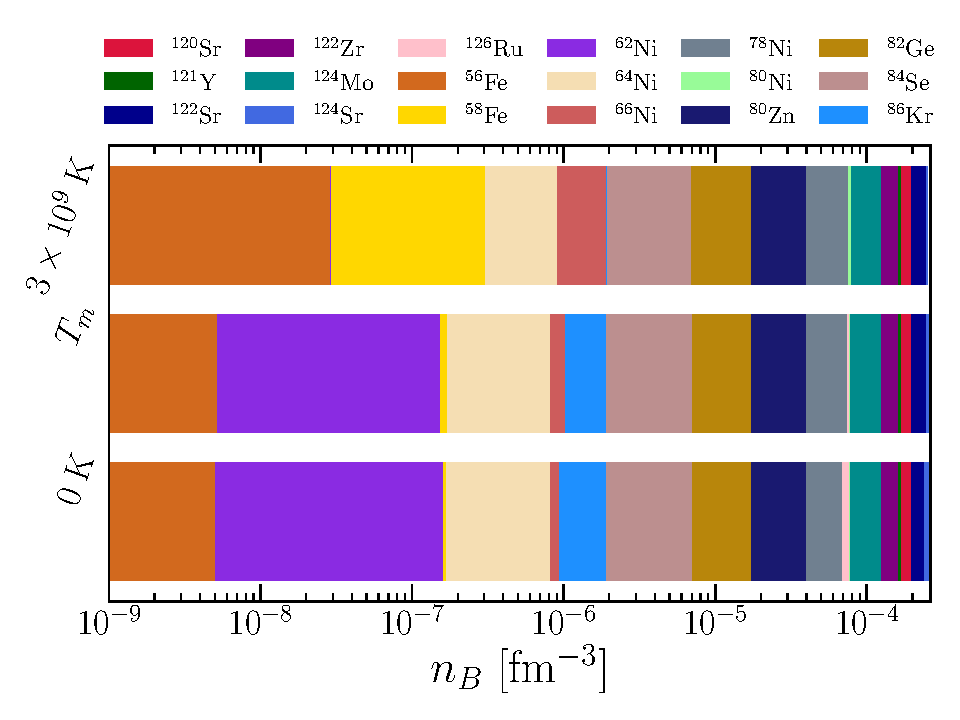
\includegraphics[width=\linewidth]{figures/ocrust_compo_vs_temp.pdf}
  \end{center}
  \caption[Equilibrium OCP composition versus baryon density in the outer crust 
  at finite temperature]{Equilibrium composition of a OCP as a function of 
    baryon density $n_B$ in the outer crust at $T=0$ K, $T=T_m$, and 
    $T=3\times 10^9$ K. 
  Experimental data are supplemented with masses from microscopic HFB-24 
  theoretical mass table~\cite{Goriely2013}.}\label{fig:ocrust_compo_vs_temp}
\end{figure}

The crystallization temperature in the outer crust does not exceed $\approx
0.25$ MeV, which is very low from the nuclear physics point of view. Hence, one
can ask whether the composition at crystallization is different to that of
CCM, presented in Section~\ref{sec:ocrust_gs}.
Fig.~\ref{fig:ocrust_compo_vs_temp} shows the equilibrium composition of a OCP
as a function of the baryon density $n_B$ in the regime of the outer crust for
two different temperatures: $T=0$ K (CCM) and $T=3\times 10^9$ K, and at 
crystallization, $T=T_m$. We make use of the microscopic HFB-24 theoretical 
mass table to complement the experimental data.
Let us notice that for all densities encountered in the outer crust, nonlinear 
mixing effects are so small that the equilibrium nucleus obtained within OCP 
approximation coincides with the most probable ion in the MCP mixture.
% discuss differences between t=0 and t=tm
We find that the difference between $T=0$ K and $T=T_m$ is very small and 
hardly visible in the figure. The exact same sequence of layers is observed in 
the two cases, only the transition densities being slightly different.
This shows that the CCM hypothesis gives an accurate description of the 
composition of the outer crust at crystallization.
% observations at larger temperatures
Significant deviations with respect to the results at $T=0$ K and $T=T_m$ are 
observed at $T=3\times 10^9$ K, which is above the crystallization temperature
in the outer crust. In particular, the layers of $^{62}$Ni and $^{86}$Kr are 
not recovered, and $^{80}$Ni is favored over $^{126}$Ru around $n_B \approx 
8\times 10^{-5}$ fm$^{-3}$.

\begin{figure}[!t]
  \begin{center}
    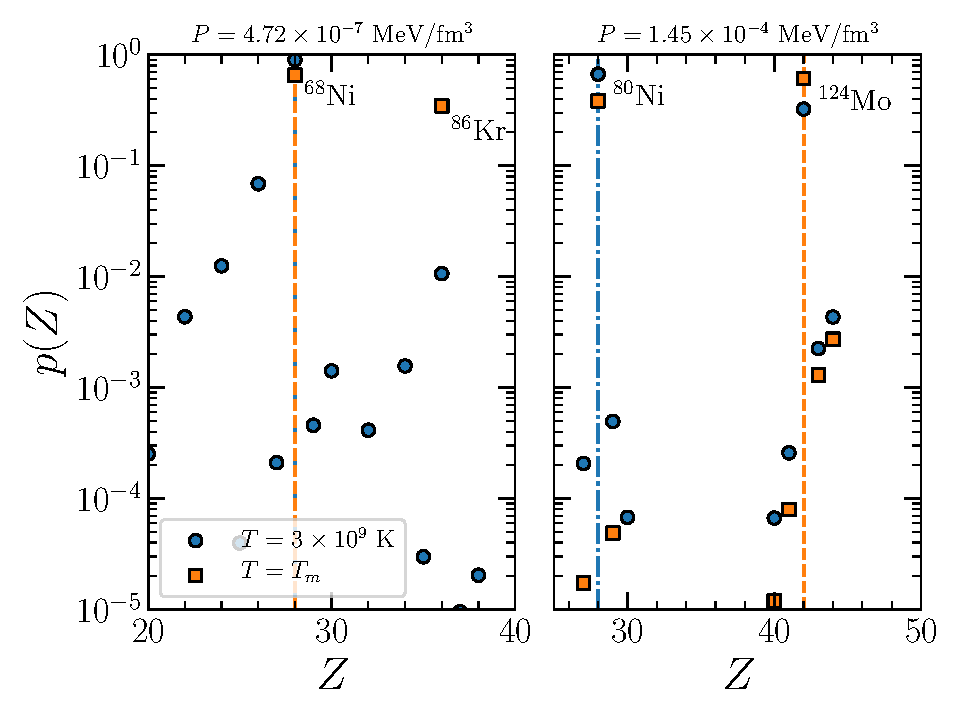
\includegraphics[width=0.9\linewidth]{figures/pj_ocrust.pdf}
  \end{center}
  \caption[Normalized probability distribution of the atomic number $Z$ for
  different thermodynamic conditions]{Normalized probability distribution 
    $p(Z)$ for $P=4.72\times 10^{-7}$ MeV/fm$^3$ (left panel) and $P=1.45\times 
    10^{-4}$ MeV/fm$^3$ (right panel) at $T=3\times 10^9$ K (blue circles) and 
    $T=T_m$ (orange squares). The blue dashdotted and orange dashed vertical 
    lines indicate the OCP solution at $T=3\times 10^9$ K and $T=T_m$,
    respectively.
    Experimental data are supplemented with masses from microscopic 
    HFB-24 theoretical mass table~\cite{Goriely2013}. 
    Figure inspired from~\cite{Fantina2020}.}\label{fig:pj_ocrust}
\end{figure}

\begin{figure}[!t]
  \begin{center}
    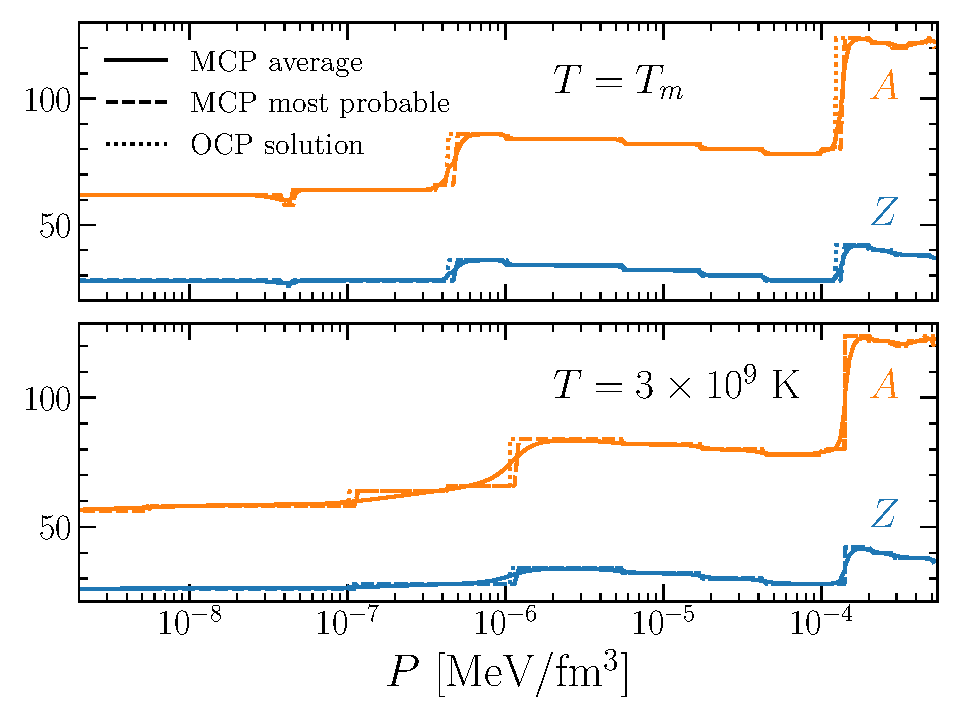
\includegraphics[width=0.9\linewidth]{figures/compo_mcp_ocrust.pdf}
  \end{center}
  \caption[Equilibrium composition of the multicomponent plasma versus pressure
  in the outer crust regime]{
    Average (solid lines) and most probable values (dashed lines) of the charge 
    number $Z$ (blue lines) and mass number $A$ (orange lines) in the MCP 
    mixture as a function of pressure in the regime of the outer crust at 
    $T=T_m$ (upper panel) and $T=3\times 10^9$ K (lower panel). 
    The OCP solution is represented in dotted lines.
    Experimental data are supplemented with masses from microscopic 
    HFB-24 theoretical mass table~\cite{Goriely2013}. 
  Figure inspired from~\cite{Fantina2020}.}\label{fig:compo_mcp_ocrust}
\end{figure}

The normalized probability distribution $p(Z)$ of the MCP mixture is 
represented in Fig.~\ref{fig:pj_ocrust} for different thermodynamic conditions 
relevant for the regime of the outer crust: $P = 4.72\times 10^{-7}$ MeV/fm$^3$
(left panel) and $P=1.45\times 10^{-4}$ MeV/fm$^3$ (right panel). For both 
selected values of pressure, we plot the distribution for $T=3\times
10^9$ K (blue circles) and for the crystallization temperature $T=T_m$ 
calculated within the OCP approximation (orange squares).
For each selected thermodynamic condition, it is observed that the most
probable $Z$ in the MCP mixture coincide with the OCP solution represented by 
a vectical line.
At low pressure, the crystallization temperature is small and consequently only 
very few configurations are expected to occur. This can be seen in the left
panel of the figure, $P = 4.72\times 10^{-7}$ MeV/fm$^3$, where only $Z=28$
($p(^{66}\text{Ni}) = 0.65$) and $Z=36$ ($p(^{86}\text{Kr})=0.35$) are 
associated to nonnegligible probabilities. This contrasts with the 
distribution calculated 
at $T=3\times 10^9$ K for the same value of pressure, for which a large number 
of configurations are found with $p(Z) > 10^{-5}$. Still, at this temperature 
the distribution is strongly peaked at $Z=28$, while for $T=T_m$ the 
distribution is bimodal. 
In the right panel of Fig.~\ref{fig:pj_ocrust}, a bimodal behavior is also 
clearly exhibited around $Z=28$ and $Z=42$, respectively corresponding to 
$^{80}$Ni and $^{124}$Mo, in the vicinity of $P = 1.45\times 10^{-4}$ 
MeV/fm$^3$, where the curve of the crystallization temperature becomes very 
steep, see Fig.~\ref{fig:tm_ocrust}. 
While $^{124}$Mo is favored over $^{80}$Ni at high temperature,
it turns out that the most probable nucleus change to $^{80}$Ni as the
temperature is decreased, and ultimately corresponds to the most probable
nucleus at the crystallization temperature. The same feature is observed for 
the OCP solution.

Fig.~\ref{fig:compo_mcp_ocrust} shows the equilibrium composition of the MCP as
a function of pressure in the regime of the outer crust at the crystallization
temperature (upper panel) and at $T=3\times 10^9$ K (lower panel). At $T=T_m$, 
it is seen that the average equilibrium values $\langle Z\rangle$ and $\langle
A\rangle$ (solid blue and orange lines, respecitvely) coincides almost 
perfectly with the OCP solution (dotted blue and orange lines), apart in the
vicinity of $P=4.5\times 10^{-7}$ MeV/fm$^3$ and $P=1.5\times 10^{-4}$
MeV/fm$^3$, where the distribution $p(Z)$ exhibits a bimodal character, as
observed in Fig.~\ref{fig:pj_ocrust}. This results in the sotening of the shell 
effects, which is even more striking at $T=3\times 10^9$ K. Those deviations 
from the OCP approximation are reflected in the Coulomb coupling parameter, 
which exhibits spikes and can be as high as $\approx 330$ at the
crystallization temperature, see Fig.~4 of~\cite{Fantina2020}.

\subsection{Impurity parameter}\label{subsec:qimp_ocrust}

% definition impurity parameter
Once the abundancies of the different ions are computed via Eq.~(\ref{eq:pj}), 
the so-called impurity parameter of the solid crust, which represents the 
variance of the ionic charge distribution, can be evaluated. It is defined
as~\cite{Meisel2018}
%
\begin{equation}
  Q_{\text{imp}} = \sum_j p(Z^{(j)})(Z^{(j)}-\langle Z \rangle)^2,
\end{equation}
%
where $p(Z^{(j)})$ represents the normalized probability distribution, that is
integrated over all $N^{(j)}$, of the atomic number $Z^{(j)}$.
% astrophysical implications of this quantity and state-of-the-art
The impurity parameter allows to quantify the presence of amorphous and
heterogeneous phases in the crust, which is expected to reduce the electrical 
conductivity of the solid crust. In consequence, the impurity
facotr is expected to play an important role in the magneto-thermal 
evolution of the star (see the discussion in Sect.~7 in~\cite{Meisel2018} for a 
review). For instance, $Q_{\text{imp}}$ is directly related to impurity 
scattering, which alters the cooling of the crust.
In NS cooling simulations, the impurity parameter is generally taken as a free 
parameter which is directly fitted to cooling data.

% FIG

% comment left panel

% comment right panel

\subsection{Abundancies of odd nuclei}\label{subsec:odd_ocrust}

\section{Study of the inner crust at crystallization}

\subsection{Influence of shell effects in the OCP
approximation}\label{subsec:shtemp}

\subsubsection{Temperature dependence of shell corrections}

\subsubsection{Equilibrium composition at crystallization for modern BSk 
functionals}

\subsection{Equilibrium composition of the MCP and the importance of the
rearrangement term}

\subsection{Dependence of the impurity parameter on the EoS}

\section{Conclusion}
